\documentclass[aspectratio=169]{beamer}

% ── Theme (same style as myos.tex) ──────────────────────────────────────────
\usetheme{Madrid}
\usecolortheme{seahorse}
\usefonttheme{professionalfonts}

% ── Packages ─────────────────────────────────────────────────────────────────
\usepackage{listings}
\usepackage{xcolor}
\usepackage{tikz}
\usepackage{booktabs}
\usepackage{hyperref}
\usepackage{textcomp}
\usepackage{microtype}

% ── Listing style ─────────────────────────────────────────────────────────────
\definecolor{codebg}{HTML}{1E1E2E}
\definecolor{codegreen}{HTML}{A6E3A1}
\definecolor{codeblue}{HTML}{89DCEB}
\definecolor{codeyellow}{HTML}{F9E2AF}
\definecolor{codegray}{HTML}{6C7086}
\definecolor{codepurple}{HTML}{CBA6F7}
\definecolor{codeorange}{HTML}{FAB387}
\definecolor{codewhite}{HTML}{CDD6F4}
\definecolor{alertred}{HTML}{F38BA8}

\lstdefinestyle{clang}{
  backgroundcolor=\color{codebg},
  basicstyle=\ttfamily\footnotesize\color{codewhite},
  keywordstyle=\color{codepurple}\bfseries,
  commentstyle=\color{codegray}\itshape,
  stringstyle=\color{codegreen},
  numberstyle=\tiny\color{codegray},
  numbers=left, numbersep=6pt,
  breaklines=true, frame=single,
  rulecolor=\color{codeblue},
  language=C,
  tabsize=4
}

\lstdefinestyle{makefile}{
  backgroundcolor=\color{codebg},
  basicstyle=\ttfamily\footnotesize\color{codewhite},
  keywordstyle=\color{codeyellow}\bfseries,
  commentstyle=\color{codegray}\itshape,
  numberstyle=\tiny\color{codegray},
  numbers=left, numbersep=6pt,
  breaklines=true, frame=single,
  rulecolor=\color{codeyellow},
  tabsize=4
}

% ── Metadata ─────────────────────────────────────────────────────────────────
\title[MyOS Chapter 2]{\textbf{MyOS Chapter 2: VGA Terminal Driver}}
\subtitle{From direct writes to a structured screen module}
\author{MyOS Project}
\date{March 2026}
\institute{Bare-metal x86, freestanding C}

% ── Helpers ──────────────────────────────────────────────────────────────────
\newcommand{\concept}[2]{%
  \begin{block}{#1}\smallskip #2\smallskip\end{block}\vspace{5pt}}

\newcommand{\warn}[1]{%
  \begin{alertblock}{Important}\smallskip #1\smallskip\end{alertblock}\vspace{5pt}}

\begin{document}

\begin{frame}
  \titlepage
\end{frame}

\begin{frame}{Chapter Goal}
  We convert kernel text output into a proper \textbf{terminal driver module}.
  \begin{itemize}
    \item Manage cursor row/column state
    \item Handle newline and line wrapping
    \item Scroll when output reaches bottom
    \item Clear screen using current color
    \item Expose simple API: \texttt{print()}, \texttt{put\_char()}, \texttt{set\_color()}
  \end{itemize}
  \vspace{6pt}
  \concept{Architecture shift}{
    \texttt{kernel.c} now expresses \textit{what} to print.\
    \texttt{screen.c} handles \textit{how} bytes are written into VGA memory.
  }
\end{frame}

\begin{frame}{VGA Text Mode Memory Model}
  \begin{columns}[T]
    \column{0.55\textwidth}
    \begin{itemize}
      \item VGA text buffer base: \texttt{0xB8000}
      \item Screen: \texttt{80 x 25} cells
      \item One cell = 2 bytes
      \begin{itemize}
        \item low byte = ASCII character
        \item high byte = color attribute
      \end{itemize}
      \item Linear index: \texttt{index = row * 80 + col}
      \item Cell value: \texttt{(color << 8) | c}
    \end{itemize}
    \column{0.42\textwidth}
    \begin{center}
    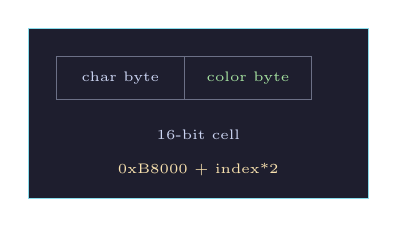
\begin{tikzpicture}[scale=0.9]
      \draw[fill=codebg,draw=codeblue] (0,0) rectangle (4.8,2.4);
      \draw[draw=codegray] (0.4,1.4) rectangle (2.2,2.0);
      \draw[draw=codegray] (2.2,1.4) rectangle (4.0,2.0);
      \node[font=\tiny,color=codewhite] at (1.3,1.7) {char byte};
      \node[font=\tiny,color=codegreen] at (3.1,1.7) {color byte};
      \node[font=\tiny,color=codewhite] at (2.4,0.9) {16-bit cell};
      \node[font=\tiny,color=codeyellow] at (2.4,0.4) {0xB8000 + index*2};
    \end{tikzpicture}
    \end{center}
  \end{columns}
\end{frame}

\begin{frame}[fragile]{Public Interface: \texttt{screen.h}}
  \begin{lstlisting}[style=clang]
#ifndef SCREEN_H
#define SCREEN_H

typedef unsigned char uint8_t;
typedef unsigned short uint16_t;

#define VGA_WIDTH 80
#define VGA_HEIGHT 25

void clear_screen();
void put_char(char c);
void print(const char* str);
void set_color(uint8_t color);

#endif
  \end{lstlisting}
  \textbf{Line logic:}
  \begin{itemize}
    \item Type aliases replace \texttt{<stdint.h>} because build uses \texttt{-nostdinc}.
    \item Constants define terminal geometry shared by all driver functions.
    \item Function list is the module contract used by \texttt{kernel.c}.
  \end{itemize}
\end{frame}

\begin{frame}[fragile]{Driver State: \texttt{screen.c}}
  \begin{lstlisting}[style=clang]
static uint16_t* video_memory = (uint16_t*) 0xB8000;

static uint8_t cursor_row = 0;
static uint8_t cursor_col = 0;
static uint8_t current_color = 0x07;
  \end{lstlisting}
  \textbf{Line logic:}
  \begin{itemize}
    \item \texttt{video\_memory} points directly to mapped hardware text RAM.
    \item Cursor state is kept private (\texttt{static}) inside the module.
    \item \texttt{current\_color = 0x07} defaults to light grey on black.
  \end{itemize}
  \vspace{4pt}
  \concept{Why static?}{
    It hides internals from other files, preventing accidental writes to cursor state.
  }
\end{frame}

\begin{frame}[fragile]{Scrolling Algorithm}
  \begin{lstlisting}[style=clang]
static void scroll() {
    if (cursor_row < VGA_HEIGHT)
        return;

    for (int row = 1; row < VGA_HEIGHT; row++) {
        for (int col = 0; col < VGA_WIDTH; col++) {
            video_memory[(row - 1) * VGA_WIDTH + col] =
                video_memory[row * VGA_WIDTH + col];
        }
    }

    for (int col = 0; col < VGA_WIDTH; col++) {
        video_memory[(VGA_HEIGHT - 1) * VGA_WIDTH + col] =
            (current_color << 8) | ' ';
    }

    cursor_row = VGA_HEIGHT - 1;
}
  \end{lstlisting}
\end{frame}

\begin{frame}{Scrolling Logic Explained}
  \begin{enumerate}
    \item Overflow check: if cursor is still inside screen, do nothing.
    \item Shift phase: copy rows \texttt{1..24} into \texttt{0..23}.
    \item Clear phase: fill last row with spaces in current color.
    \item Re-anchor cursor: set row to \texttt{VGA\_HEIGHT - 1}.
  \end{enumerate}
  \vspace{6pt}
  \concept{Complexity}{
    One scroll touches \texttt{80 * 25 = 2000} cells worst-case, which is fine for early boot text output.
  }
\end{frame}

\begin{frame}[fragile]{Character Path: \texttt{put\_char}}
  \begin{lstlisting}[style=clang]
void put_char(char c) {
    if (c == '\n') {
        cursor_col = 0;
        cursor_row++;
        scroll();
        return;
    }

    video_memory[cursor_row * VGA_WIDTH + cursor_col] =
        (current_color << 8) | c;

    cursor_col++;

    if (cursor_col >= VGA_WIDTH) {
        cursor_col = 0;
        cursor_row++;
        scroll();
    }
}
  \end{lstlisting}
  \textbf{Line logic:}
  \begin{itemize}
    \item Newline is a control path: advance row, reset col.
    \item Normal chars pack color+ASCII into one 16-bit write.
    \item End-of-line wrap reuses same row increment + scroll path.
  \end{itemize}
\end{frame}

\begin{frame}[fragile]{String and Color Helpers}
  \begin{lstlisting}[style=clang]
void print(const char* str) {
    int i = 0;
    while (str[i]) {
        put_char(str[i]);
        i++;
    }
}

void set_color(uint8_t color) {
    current_color = color;
}

void clear_screen() {
    for (int i = 0; i < VGA_WIDTH * VGA_HEIGHT; i++) {
        video_memory[i] = (current_color << 8) | ' ';
    }
    cursor_row = 0;
    cursor_col = 0;
}
  \end{lstlisting}
\end{frame}

\begin{frame}{Why these helpers matter}
  \begin{itemize}
    \item \texttt{print()} keeps all cursor rules centralized inside \texttt{put\_char()}.
    \item \texttt{set\_color()} updates global terminal style for subsequent output.
    \item \texttt{clear\_screen()} resets both hardware cells and logical cursor state.
    \item Using one module API prevents duplicated VGA logic across kernel files.
  \end{itemize}
\end{frame}

\begin{frame}[fragile]{Kernel Integration (Policy Layer)}
  \begin{lstlisting}[style=clang]
#include "screen.h"

void kernel_main() {
    clear_screen();

    set_color(0x0A);
    print("=================================\n");
    print("        MyOS v0.1\n");
    print("=================================\n\n");

    set_color(0x07);
    print("Screen driver initialized.\n");
    print("Scrolling works.\n");
    print("New lines work.\n");

    while (1);
}
  \end{lstlisting}
\end{frame}

\begin{frame}[fragile]{Build Changes for New Module}
  \begin{lstlisting}[style=makefile]
KERNEL_C := kernel/kernel.c
SCREEN_C := kernel/screen.c

$(BUILD)/kernel.o: $(KERNEL_C) | $(BUILD)
	$(CC) $(CFLAGS) -c $< -o $@

$(BUILD)/screen.o: $(SCREEN_C) | $(BUILD)
	$(CC) $(CFLAGS) -c $< -o $@

$(BUILD)/kernel.bin: $(BUILD)/kernel_entry.o $(BUILD)/kernel.o $(BUILD)/screen.o
	$(LD) $(LDFLAGS) -o $@ $^ --oformat binary
  \end{lstlisting}
  \warn{Freestanding toolchain note: with \texttt{-nostdinc}, include your own fixed-width typedefs or provide minimal headers.}
\end{frame}

\begin{frame}{What Chapter 2 Delivers}
  \begin{itemize}
    \item First real kernel subsystem: a reusable terminal driver
    \item Deterministic behavior for newline, wrapping, and scrolling
    \item Cleaner kernel architecture through module boundaries
    \item Foundation for next upgrades: hardware cursor, \texttt{printk}, keyboard input
  \end{itemize}
  \vspace{8pt}
  \begin{center}
    \Large \textbf{Chapter 2 Complete: VGA Terminal Module Online}
  \end{center}
\end{frame}

\end{document}
